\documentclass[letterpaper,11pt]{article}

% Soporte para los acentos.
\usepackage[utf8]{inputenc}
\usepackage[T1]{fontenc}
% Idioma español.
\usepackage[spanish,mexico, es-tabla]{babel}
% Soporte de símbolos adicionales (matemáticas)
\usepackage{multirow}
\usepackage{amsmath}
\usepackage{amssymb}
\usepackage{amsthm}
\usepackage{amsfonts}
\usepackage{mathtools}
\usepackage{latexsym}
\usepackage{enumerate}
\usepackage{ragged2e}
\usepackage{listings}
\usepackage{xcolor}
\usepackage{graphicx}
\usepackage{hyperref}
\usepackage[linguistics]{forest}
\usepackage{algorithm}
\usepackage{algpseudocode}

% Modificamos los márgenes del documento.                                       
\usepackage[lmargin=2cm,rmargin=2cm,top=2cm,bottom=2cm]{geometry}

\title{Facultad de Ciencias, UNAM \\ 
       Análisis de Algoritmos \\ 
       Tarea 1}
\author{Rubí Rojas Tania Michelle}
\date{14 de octubre de 2020}

\begin{document}
\maketitle

\begin{enumerate}
    % Ejercicio 1.
    \item ¿Cuántas comparaciones son necesarias y suficientes para ordenar 
    cualquier lista de cinco elementos? Justifique su respuesta.

    \textsc{Solución:} Un árbol de decisión es un árbol binario completo que 
    representa las comparaciones realizadas en todas las ejecuciones posibles 
    sobre entradas de tamaño $n$. Cada nodo interno se representa de la forma 
    $i:j$ con $1 \leq i < j \leq n$ y cada hoja con una permutación 
    $\langle \pi(1), \pi(2), ..., \pi(n) \rangle$ sobre $\{1, 2, ..., n\}$.

    La ejecución del algoritmo de ordenamiento sobre una entrada dada 
    corresponde a un camino en el árbol desde la raíz hasta la hoja. Dicho 
    camino denota las comparaciones realizadas y su órden de realización para 
    la entrada. Es decir, un nodo $i:j$ en el camino denota la comparación 
    $a_i \leq a_j$. Si el camino continúa sobre el hijo izquierdo, la
    comparación es cierta y si continúa sobre el hijo derecho entonces la 
    comparación es falsa. Si la entrada alcanza la hoja $\langle \pi(1), 
    \pi(2), ..., \pi(n) \rangle$, entonces la permutación de entrada ordenada 
    es $\langle a_{v\pi(1)}, a_{\pi(2)}, ..., a_\pi(n) \rangle$.

    Un ejemplo de árbol de decisión sería el siguiente:
    \begin{figure}[h]
        \centering
        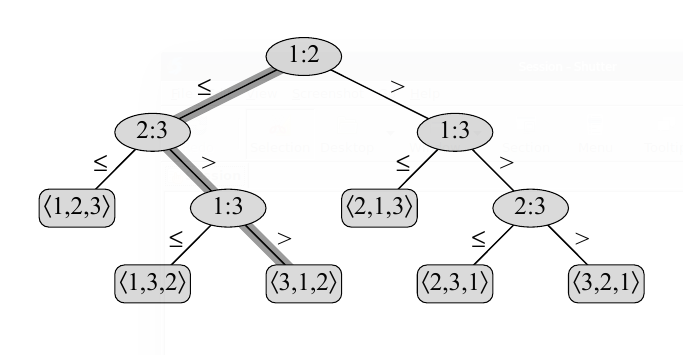
\includegraphics[width=0.5\linewidth]{imagenes/decision-tree.png}
        \caption{Árbol de decisión correspondiente a tres elementos (Cormen, 
        pag. 192)}
        \label{fig:decision-tree}
    \end{figure}

    La entrada corresponde a $\langle a_1, a_2, a_3 \rangle = \langle 6, 8, 5, 
    \rangle$. Lo primero que hace es la comparación $a_1 \leq a_2$, que es 
    cierta. Luego se compara $a_2 \leq a_3$, que es falsa. Finalmente compara 
    $a_1 \leq a_3$, que también es falsa. La entrada ordenada es $\langle 5, 6, 
    8 \rangle$. Notemos que hay $3! = 6$ posibles permutaciones en la entrada 
    de elementos, por lo que el árbol de decisión tiene $6$ hojas.

    Ahora bien, de manera más general, digamos que para $n$ elementos tenemos 
    un árbol de decisión $T$ de altura $h$ y con $l$ hojas alcanzables. Como el 
    árbol ordena las $n!$ distintas permutaciones, entonces el árbol contiene 
    una hoja por cada una de las $n!$ permutaciones, por lo que $n! \leq l$. 
    Como un árbol binario de altura $h$ tiene a lo más $2^h$ hojas, entonces 
    $n! \leq l \leq 2^h$, de donde 
    \begin{align*}
        2^h &\geq n!
        && \text{por transitividad} \\
        \log_2 (2^h) &\geq \log_2 (n!)
        && \text{tomando los logaritmos} \\
        h &\geq \log_2 (n!)
        && \text{propiedad de logaritmo} \\
        &= \log_2 (n \cdot (n-1) \cdot (n-2) \cdot (n-3) \cdots \cdot 3 \cdot 
        2 \cdot 1)
        && \text{definición de factorial} \\ 
        &= \log_2 (n) + \log_2 (n-1) + \log_2 (n-2) + \log_2 (n-3) +
        && \text{propiedad de logaritmo} \\ 
        & \; \; \; \; \;  \cdots + \log_2 (3) + \log_2 (2) + \log_2 (1) \\
        &= \int_1^n \! \log_2 (x) \, \mathrm{d}x.
        && \text{es el área bajo la curva} \\ 
        &= x \log_2 (x) - x \Big|_1^n
        && \text{resolvemos la integral}
    \end{align*}

    Es decir, para poder ordenar un arreglo de $n$ elementos son 
    \texttt{necesarias} y \texttt{suficientes} 
    \begin{equation*}
        h = x \log_2 (x) - x \Big|_1^n
    \end{equation*}

    comparaciones. ¿Por qué? Esto se debe a que el árbol de decisión ya contempla 
    las $n!$ permutaciones de nuestro arreglo y éstas se encuentran en las hojas 
    del árbol, así que para acceder a ellas necesitamos recorrer (en un peor caso, 
    si se quiere ver así) toda la altura del árbol. Son \texttt{suficientes} porque 
    si agregamos un nivel al árbol, realmente no estamos obteniéndo información 
    nueva (sino repetida) pues el árbol ya se encargó de contemplar todas las 
    comparaciones que necesitamos. Ahora bien, son \texttt{necesarias} porque si 
    eliminamos un nivel al árbol entonces estamos eliminando comparaciones que son 
    realmente de utilidad, por lo que como mínimo debemos tener ese número de 
    comparaciones.

    En particular, si $n = 5$ entonces tendríamos que son \texttt{necesarias} y 
    \texttt{suficientes}
    \begin{equation*}
        h = 5 \log_2 (5) - 5 \Big|_1^5 = 7
    \end{equation*} 
    
    comparaciones.

    \newpage
    % Ejercicio 2.
    \item Dados dos arreglos ordenados $A$ y $B$ de longitud $n$ y $m$, 
    respectivamente. Diseña un algoritmo de tiempo $O(n + m)$ que obtenga un 
    arreglo $C$ que contenga los elementos en común entre $A$ y $B$, $C$ no 
    debe tener elementos repetidos.

    \textsc{Solución:} El algoritmo propuesto para resolver este problema es 
    el siguiente
    \begin{center}
    \begin{minipage}[c]{0.7\textwidth}
    \begin{algorithm}[H]
        \caption{Obtener los elementos en común entre los arreglos $A$ y $B$ \\
                 encontrarInterseccion(A, B): } 
        \begin{algorithmic}[1]
            \State $i \gets 0$
            \State $j \gets 0$
            \State $C = []$
            \While {$(i < n$ \textbf{and} $j < m)$}
                \If {$A[i] == B[j]$}
                    \If {$C.length > 0$ \textbf{and} $C[C.length - 1] == A[i]$}
                        \State $i \gets i + 1$
                        \State $j \gets j + 1$
                    \Else
                        \State $C.append[A[i]]$
                        \State $i \gets i + 1$
                        \State $j \gets j + 1$
                    \EndIf
                \Else \If {A[i] < B[j]}
                    \State $i \gets i + 1$
                \Else
                    \State $j \gets j + 1$
                \EndIf
                \EndIf
            \EndWhile

            \State return $C$
        \end{algorithmic} 
    \end{algorithm}
    \end{minipage}
    \end{center}
   
    Primero, explicaremos porqué el algoritmo funciona. En las líneas $(1 - 2)$ 
    estamos definiéndo dos variables $i, j$; las cuales nos ayudarán a recorrer
    los arreglos $A$ y $B$, respectivamente. En la línea $3$ simplemente creamos 
    a nuestro arreglo $C$. A partir de la línea $4$ empieza lo interesante: como
    sabemos que los arreglos $A$ y $B$ están ordenados, eso significa que 
    tenemos que checar tres casos en específico:
    \begin{enumerate}
        \item (líneas $(5 - 13)$). Si el $i-$ésimo elemento de $A$ es igual al 
        $j-$ésimo elemento de $B$ eso significa que tienen un elemento en común 
        y, en teoría, se debe agregar al arreglo $C$. Pero antes de agregarlo,
        comprobamos que no esté repetido en $C$: para verificar esto simplemente
        hay que ver si el elemento $A[i]$ (o $B[j]$) es igual al último elemento 
        que fue agregado a $C$ (como $A$ y $B$ están ordenados, si es que tienen 
        elementos repetidos, entonces éstos están juntos). Si el elemento ya se 
        encuentra en $C$ entonces simplemente incrementamos nuestros contadores 
        en \textit{uno}; en caso contrario, agregamos al elemento a $C$ e 
        incrementamos los contadores en \textit{uno}.

        \item (líneas $(15 - 16)$). Si el $i-$ésmo elemento de $A$ es menor que 
        el $j-$ésimo elemento de $B$, eso quiere decir que debemos movernos un 
        índice a la derecha en el arreglo $A$; ya que como están ordenados ambos 
        arreglos, eso quiere decir que, si tienen elementos en común, entonces 
        éste (o éstos) es mayor que el $i-$ésimo elemento de $A$.

        \newpage
        \item (línea $18$). Aquí cae el caso en que $B[j] < A[i]$, y 
        análogamente al caso anterior, tenemos que movernos un índice a la 
        derecha en el arreglo $B$; ya que como están ordenados ambos arreglos, 
        eso quiere decir que, si tiene elementos en común, entonces éste (o 
        éstos) es mayor que el $j-$ésimo elemento de $B$. 
    \end{enumerate} 

    Todo esto se realizará hasta que la condición de nuestro \textit{while} 
    (línea $14$) se cumpla: como $n$ puede ser diferente de $m$,
     lo que hay 
    que tener en cuenta es que si terminamos de recorrer un arreglo, entonces 
    debemos terminar el proceso. Esto se debe al hecho de que los arreglos
    están ordenados. Si terminamos de recorrer un arreglo, entonces ya no 
    habrá más elementos en común, es decir, podríamos recorrer un arreglo sin 
    terminar de recorrer al otro; pero en el peor caso, debemos recorrer 
    completamente ambos arreglos, por este motivo la complejidad de nuestro 
    algoritmo es $O(n + m)$. En particular, porque sólo estamos recorriéndo los 
    arreglos y las demás operaciones que realizamos se hacen en tiempo constante.

    % Ejercicio 3.
    \item Consider the following sorting algorithm:
    \begin{figure}[ht]
        \centering
        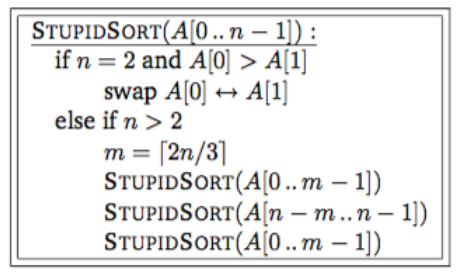
\includegraphics[width=0.4\textwidth]{./imagenes/stupidSort.png}
    \end{figure}

    \begin{enumerate}
        % Ejercicio 3.1
        \item Prove that \textsc{stupidsort} actually sorts its input.
        \begin{proof}
            Inducción fuerte sobre la longitud $n$ del arreglo. 
            \begin{itemize}
                \item \textbf{Caso base}
                
                $n = 1$. El arreglo ya está ordenado, así que no hay nada más 
                que hacer. 

                $n = 2$. Aquí tenemos dos posibles casitos:
                \begin{enumerate}
                    \item $A[0] < A[1]$. No se contempla como tal en el
                    algoritmo, pero seguramente es porque esto significa que 
                    el arreglo ya está ordenado y no hay nada más que hacer.

                    \item $A[0] > A[1]$. En este  caso, como el elemento menor 
                    se encuentra al final del arreglo, entonces intercambiamos 
                    las posiciones del primer y último elemento con ayuda del 
                    \texttt{swap}; y así obtenemos que el algoritmo ordena 
                    este caso, y por lo tanto se cumple. 
                \end{enumerate}

                \item \textbf{Hipótesis de inducción}

                Supongamos que el algoritmo \textsc{StupidSort} ordena todos 
                los arreglos de longitud $k$ que sean menores a $n$. 

                \item \textbf{Paso inductivo}

                Primero, mostraremos que $\lceil \frac{2n}{3} \rceil < n$ para 
                $n > 2$.
                \begin{proof}
                    Inducción sobre $n$.
                    \begin{itemize}
                        \item \textbf{Caso base}

                        $n = 3$. Este caso se cumple ya que 
                        \begin{align*}
                            \Big \lceil \frac{2(3)}{3} \Big \rceil &< 3 \\
                            \lceil 2 \rceil &< 3 \\ 
                            2 &< 3
                        \end{align*}

                        \item \textbf{Hipótesis de inducción}

                        Supongamos que se cumple para $n > 2$, es decir, que se 
                        cumple $\lceil \frac{2n}{3} \rceil < n$.  

                        \item \textbf{Paso inductivo}
                        
                        Queremos mostrar que se cumple para $n+1$, es decir, 
                        que se cumple $\lceil \frac{2(n+1)}{3} \rceil < n+1$. 
                        Entonces 
                        \begin{align*}
                            \Big \lceil \frac{2(n+1)}{3} \Big \rceil
                            &= \Big \lceil \frac{2n + 2}{3} \Big \rceil  
                            && \text{aritmética} \\
                            &= \Big \lceil \frac{2n}{3} + \frac{2}{3} \Big \rceil
                            && \text{propiedad de fracciones} \\
                            &< \Big \lceil n + \frac{2}{3} \Big \rceil
                            && \text{por H.I} \\
                            &< \lceil n + 1 \rceil
                            && \text{ya que $\frac{2}{3} < 1$} \\
                            &< n + 1
                        \end{align*}

                        Por lo tanto, $\lceil \frac{2n}{3} \rceil < n$ para
                        $n > 2$.
                    \end{itemize}
                \end{proof}

                Sea $n > 2$. Como $m - 1 < n$, por hipótesis de inducción, tenemos 
                que el subarreglo $A[0 \ldots m-1]$ es ordenado satisfactoriamente 
                por \textsc{stupidsort}. La siguiente llamada recursiva se realiza 
                sobre el subarreglo $A[n-m \ldots n-1]$ y queremos ver qué pasa 
                con los índices del subarreglo $A[0 \ldots m-1]$ con respecto a los 
                índices del subarreglo $A[n-m \ldots n-1]$ en esta segunda llamda 
                recursiva; por lo que vamos a considerar dos casos:
                \begin{enumerate}
                    \item $m - 1 < n - m$

                    Este caso no puede ocurrir, puesto que antes mostramos que 
                    $m < n$ para $n > 2$; lo cual implica que $m - 1 \not < n - m$.

                    \item $m - 1 \geq n - m$

                    Aquí los índices de los subarreglos se intersectan, ya que
                    si $m - 1 = n - m$, como $n > 2$, significa que tendrán un 
                    índice en común; mientras que si $n - m < m - 1$ entonces 
                    tendrán más de un índice en común, a saber, $m-(n-m) = 2m - n$
                    índices. Como la longitud del subarreglo $A[n-m \ldots n-1]$ 
                    es $n - (n - m) = m$ entonces podemos aplicarle la hipótesis 
                    de inducción para para ordenarlo. Finalmente, en caso de que 
                    haga falta ordenar más elementos (es decir, que los elementos 
                    en esa intersección tengan que ser reacomodados) el algoritmo 
                    hace una última llamada recursiva nuevamente sobre el 
                    subarreglo $A[0 \ldots m-1]$, el cual también será ordenado 
                    por hipótesis de inducción. Así, nuestro arreglo quedará 
                    ordenado correctamente.
                \end{enumerate}
            \end{itemize}

            Por lo tanto, el algoritmo \textsc{stupidSort} ordena su entrada de 
            manera correcta.

        \end{proof}

        % Ejercicio 3.2
        \item Would the algorithm still sort correctly if we replaced 
        $m = \lceil \frac{2n}{3}\rceil$ with $m = \lfloor \frac{2n}{3} \rfloor$. 
        Justify your answer.

        \textsc{Solución:} No ordena correctamente si tomamos el piso al momento 
        de calcular $m$. Para mostrar esto, exhibiremos un contraejemplo:

        Si $A = [5, 2, 1, 4]$ entonces $n = 4$ y $m = \lfloor \frac{2(4)}{3} 
        \rfloor = 2$. Entonces,
        \begin{itemize}
            \item \texttt{STUPIDSORT(A[0..1])}

            Esta llamada de \textsc{stupidsort} toma los elementos que se 
            encuentran en azul en el arreglo $[$\textcolor{blue}{$5,2$}$,1,4]$ 
            y lo regresa acomodado de la forma $[$\textcolor{blue}{$2,5$}$,1,4]$.

            \item \texttt{STUPIDSORT(A[2..3])}

            Esta llamada de \textsc{stupidsort} toma los elementos que se 
            encuentran en azul en el arreglo $[2,5,$\textcolor{blue}{$1,4$}$]$
            y lo regresa acomodado de la forma $[2,5,$\textcolor{blue}{$1,4$}$]$.

            \item \texttt{STUPIDSORT(A[0..1])}
            
            Esta llamada de \textsc{stupidsort} toma los elementos que se 
            encuentran en azul en el arreglo $[$\textcolor{blue}{$2,5$}$,1,4]$ 
            y lo regresa acomodado de la forma $[$\textcolor{blue}{$2,5$}$,1,4]$
        \end{itemize}

        Por lo tanto, el arreglo final que nos regresa \textsc{stupidsort} es 
        $[2, 5, 1, 4]$. Como 
        \begin{equation*}
            m - 1 =  2- 1 = 1 < 2 = 4 - 2 = n - m
        \end{equation*}

        eso quiere decir que los índices de nuestros subarreglos \texttt{A[0..1]}
        y \texttt{A[2..3]} nunca se interseccionan pues el arreglo lo estaríamos 
        tratando de la forma \texttt{A[0..k, k+1..n-1]}, donde $k = m - 1$ y 
        $k+1 = n-m$. En este caso, por hipótesis de inducción los subarreglos 
        \texttt{A[0..1]} y \texttt{A[2..3]} sí serían ordenados correctamente,
        pero justo como no se intersectan, al momento de querer ordenar de nuevo 
        al subarreglo \texttt{A[0..1]}, el algoritmo no va a modificar al resto 
        del arreglo y esto nos lleva a un arreglo no ordenado.

        % Ejercicio 3.3
        \item Show that the number of swaps executed by \textsc{stupidsort} is
        at most $\big(\begin{smallmatrix} n \\ 2 \end{smallmatrix}\big)$.

        \begin{proof}
            Sabemos que si $n = 2$, en caso de que estén desordenados, entonces 
            el algoritmo realizará a lo más $1$ swap. En particular, notemos que 
            \textsc{stupidsort} sólo realizará swaps en pares de elementos 
            cuyos índices sean consecutivos y que estén desordenados, es decir, 
            en pares de elementos de la forma $A[i], A[i+1]$ con $A[i] > A[i+1]$.
            El peor caso que podemos tener es cuando nuestro arreglo $A$ está 
            ordenado al revés, entonces el número de intercambios requerido para 
            ordenarlo es exactamente $\big(\begin{smallmatrix} n \\ 2 
            \end{smallmatrix}\big)$ ya que cada dos elementos $i, j$ con $i > j$
            serán eventualmente adyacentes en el arreglo y serán intercambiados.

        \end{proof}
    \end{enumerate}

    % Ejercicio 4.
    \item Supongamos que tenemos que ordenar una lista $L$ de $n$ enteros cuyos
    valores están entre $1$ y $m$. Pruebe que si $m$ es $O(n)$ entonces los 
    elementos de $L$ pueden ser ordenados en tiempo lineal. ¿Qué pasa si $m$ es 
    de $O(n^2)$? ¿Se puede realizar en tiempo lineal? ¿Por qué?

    \begin{proof}
        Supongamos que $m$ es $O(n)$. Para probar nuestra primera interrogante,
        nos auxiliaremos del algoritmo de ordenamiento \textit{Counting Sort}.
        Éste supone que cada uno de los $n$ elementos de entrada es un natural
        en un rango de a lo más $k$. El objetivo de este algoritmo es 
        determinar, para cada elemento de entrada $x$, el número de elementos 
        que son menores a $x$. Esto es usado para colocar a $x$ en la posición 
        adecuada de salida del arreglo. En el algoritmo de \textit{Counting 
        Sort} suponemos que la entrada es el arreglo $A_{[1...n]}$ y que su 
        longitud es $n$. Además, necesitamos de dos arreglos extra: 
        $B_{[1...n]}$ que tiene los elementos ordenados, y $C_{[0...k]}$ que 
        sirve como almacenamiento temporal. Hay que tener en cuenta que este 
        algoritmo nunca hace comparaciones, sino que usa los valores de los 
        elementos para indicar las posiciones en el arreglo.

        \begin{figure}[h]
            \centering
            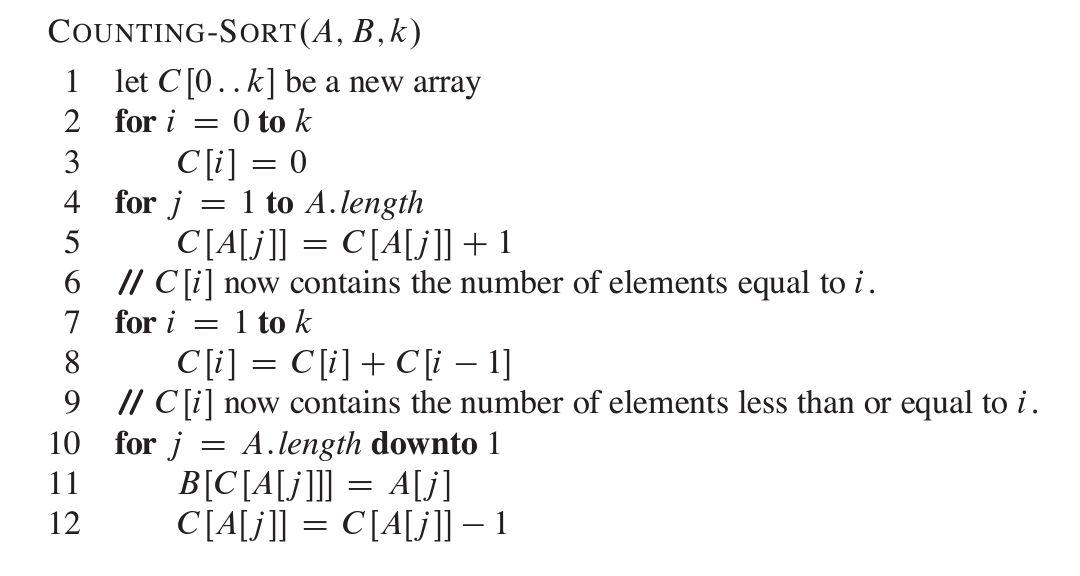
\includegraphics[width=0.55\linewidth]
            {imagenes/counting-sort-normal.jpeg}
            \caption{Algoritmo Counting Sort (Cormen, pag. 195)}
            \label{fig:counting-sort-normal}
        \end{figure}

        Las líneas $(2 - 3)$ inicializan al arreglo $C$ (creado en la línea $1$)
        con todas sus entradas en $0$. Este proceso nos toma $\Theta(k)$. En las 
        líneas $(4 - 5)$ revisamos cada elemento del arreglo. Si el valor de 
        un elemento es igual a $i$, entonces incrementamos $C_{[i]}$. Así, 
        después de la línea $5$ obtenemos el número de elementos de $A$ que son 
        iguales a cada $i \in \{0, 1, ..., k\}$. Como tenemos que recorrerlo 
        todo, entonces este proceso nos toma $\Theta(n)$. Las líneas $(7 - 8)$ 
        determinan, para cada $i \in \{0, 1, ..., k\}$, cuántos elementos de 
        $A$ son menor o iguales a $i$, al estar realizando una suma 
        \textit{corrida} entre los elementos de $C$. Nuevamente, como estamos 
        recorriendo todo el arreglo $C$, este proceso nos toma $\Theta(k)$. 
        Finalmente, las líneas $(10 - 12)$ colocan a cada elemento $A[j]$ en 
        la correcta posición que le corresponde para que esté ordenado, y esta 
        colocación se hará en el arreglo $B$. Como recorremos a todo nuestro
        arreglo $A$, eso quiere decir que este proceso nos toma $\Theta(n)$. 
        Por lo tanto, la complejidad del algoritmo \textit{Counting Sort} es 
        $\Theta(k + n)$. Así, por lo anterior, si $k = O(n)$, esto quiere 
        decir que $T(n) = n$, y por lo tanto el algoritmo será lineal. 

        Cuando $m$ es $O(n^2)$, también es posible ordenarlo en $O(n)$. Para 
        ello, utilizaremos una variación de \texttt{Radix Sort}, el cual 
        también hemos discutido en clase. La idea de \texttt{Radix} es ordenar
        dígito por dígito, empezando por el dígito menos significativo y 
        pasando al más significativo. Aquí, \texttt{Counting Sort} se usa como 
        una subrutina para ordenar. Para usar este algoritmo debe haber $d$ 
        digitos en los enteros de entrada. Usualmente, \texttt{Radix Sort} toma 
        $O(d \cdot (n + k))$, donde $k$ es la base para representar números 
        (por ejemplo, la base decimal). Como $m = O(n^2)$, entonces ese es su 
        mayor valor posible, por lo que $d = O(\log_k n)$. Así, la complejidad 
        sería $O((\log_k n) \cdot (n + k))$. Para hacer esto lineal, el truco 
        está en cambiar la base $k$. Si reemplazamos a $k$ con $n$, entonces 
        el valor de $O(\log_k n)$ se convierte en $O(1)$, y la complejidad se 
        convierte en $O(n)$. 

    \end{proof}

    % Ejercicio 5.
    \item Describe an algorithm that, given $n$ integers in the range $0$ to 
    $k$, preprocesses its input and then answers any query about how many of 
    the $n$ integers fall into a range $[a ... b]$ in $O(1)$ time. Your 
    algorithm should use $\Theta(n + k)$ preprocessing time.

    \textsc{Solución:} La solución propuesta es utilizar las líneas $(1 - 9)$
    del algoritmo \textit{Counting Sort} para preprocesar los $n$ enteros en 
    el rango $0$ a $k$.

    \begin{figure}[h]
        \centering
        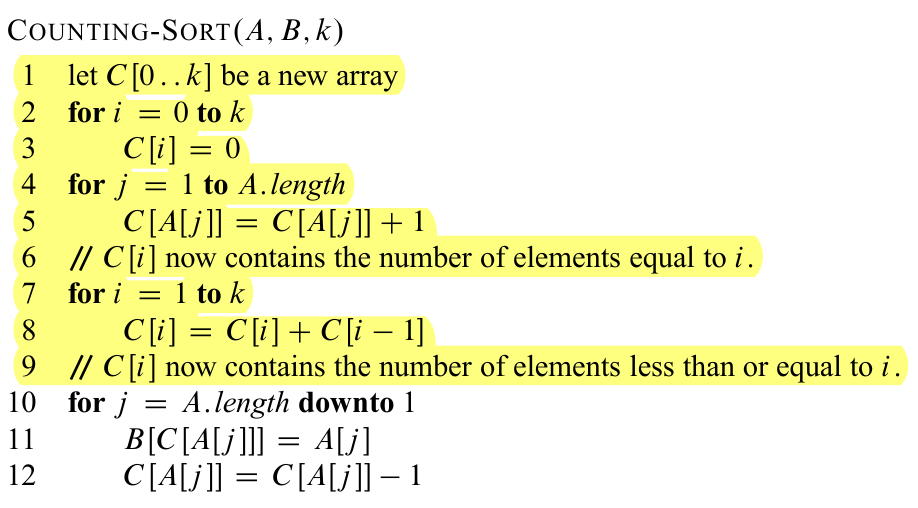
\includegraphics[width=0.5\linewidth]{imagenes/counting-sort.png}
        \caption{Algoritmo Counting Sort (Cormen, pag. 195)}
        \label{fig:counting-sort}
    \end{figure}

    Por el análisis visto en el inciso anterior, sabemos que esto se hace en 
    $\Theta(k + n)$. 

    Ahora, tenemos un arreglo $C_{[0...k]}$ en donde cada $C_{[i]}$ contiene el 
    número de enteros que son menores o iguales a $i$, por lo que el número de 
    enteros en el rango $[a...b]$ es $C_{[b]} - C_{[a-1]}$, donde podemos 
    interpretar a $C_{[-1]}$ como $0$. Esto último toma $O(1)$ porque lo único 
    que hacemos es acceder a dos elementos en el arreglo $C$ (sabemos que esto 
    es constante) y posteriormente restar. 

    % Ejercicio 6.
    \item Sea $A$ un arreglo de $n$ elementos, tal que cada elemento se 
    encuentra a lo más a $k$ posiciones de su posición ordenada. Diseñe un 
    algoritmo que ordene $A$ en $O(n \log k)$.

    \textsc{Solución:} El algoritmo propuesto es el siguiente 
    \begin{center}
        \begin{minipage}[c]{0.75\textwidth}
        \begin{algorithm}[H]
            \caption{Ordenar un arreglo cuyos elementos se encuentran a lo más 
                     $k$ posiciones de su posición correcta. \\ 
                     ordenaArreglo(A, k):} 
            \begin{algorithmic}[1]
                \State $T \gets creaMinHeap(A, k+1)$
                \State $T \gets$ T.actualizaMinimo
                \State $i \gets 0$
                \State $j \gets k + 1$

                \While{$i \leq A.length - 1$}
                    \State $A[i] \gets$ T.getRaiz
                    \State $i \gets i + 1$
                    \State $T \gets$ T.eliminaMinimo()
                    \If{$j < A.length - 1$}
                        \State $j \gets j +1$
                        \State $T \gets$ T.agregaElemento(A[j])
                    \EndIf
                \EndWhile

                \State return $A$
            \end{algorithmic} 
        \end{algorithm}
        \end{minipage}
    \end{center}

    Primero, explicaremos por qué el algoritmo funciona. Como los elementos del 
    arreglo $A$ se encuentran a lo más $k$ posiciones de su posición correcta,
    entonces el elemento más pequeño se debería encontrar en el subarreglo 
    de longitud $k+1$, ya que en el peor caso, éste se encuentra justo a $k$ 
    posiciones de su posición correcta; y al tomar el subarreglo con los 
    elementos $k+1$ entonces nos aseguramos de tomar al elemento más pequeño
    (y en caso de que esté antes de la posición $k$ entonces de todas formas 
    lo estamos agarrando). Tomando este subarreglo de longitud $k+1$ vamos a 
    crear un árbol, en particular un \texttt{MinHeap}, por lo que éste tendrá 
    $k+1$ elementos. La línea $(1)$ justo esto es lo que hará: 
    \texttt{creaMinHeap} creará un minHeap (por lo general se usa un arreglo) de 
    tamaño $k+1$ y se agregarán los primeros $k+1$ elementos de $A$ en el árbol.
    Una vez que ya tengamos el \texttt{minHeap}, lo que haremos es subir al 
    elemento más pequeño a la raíz del árbol (como se mencionó al inicio, ya 
    tenemos garantizado que el elemento más pequeño de $A$ se encuentra dentro 
    del \texttt{minHeap}). Esto se realiza durante la línea $(2)$, y las líneas 
    $(3 - 4)$ simplemente inicializan contadores que nos ayudarán a saber cuándo 
    terminar ciertas partes del algoritmo.
    
    Ahora bien, comenzamos con la parte más interesante: como ya tenemos al 
    elemento más chiquito en la raíz del árbol, entonces cambiámos al elemento 
    que se encuentra en la $i$-ésima posición del arreglo original por el 
    elemento que se encuentra en la raíz del \texttt{minHeap} y aumentamos 
    nuestro contador. Luego, eliminamos al elemento más pequeño (y esto en el 
    algoritmo de los \texttt{minHeap} implica que además de eliminar al elemento, 
    actualiza al árbol para mantener en todos sus nodos la definición de 
    \texttt{minHeap}, por lo que en particular tendremos al nuevo elemento más 
    chico en la raiz del árbol). El contador $j$ nos ayudará a ir 
    agregando a los elementos del arreglo $A$ que nos faltaron por incluir en 
    el \texttt{minHeap}, es decir, los elementos que estaban después de la 
    posición $k+1$. Entonces, si aún nos falta agregar elementos del arreglo $A$, 
    aumentamos el contador $j$ y agregamos al \texttt{minHeap} el elemento que 
    se encuentra en la entrada $j$-ésima del arreglo original (y al igual que 
    cuando eliminamos, se debe actualizar el árbol para mantener la definición 
    de \texttt{minHeap} en todos sus nodos). De igual manera, como cada elemento 
    está a lo más $k$ posiciones de su posición correcta, al ir agregando de 
    uno en uno los elementos que nos faltan del arreglo original, entonces 
    seguimos garantizando que el más pequeño se encuentra dentro del 
    \texttt{minHeap}. Todo esto se realiza en las líneas $(6 - 12)$. Así,
    vamos a ir realizando este proceso hasta que agreguemos todos los elementos
    de $A$ en el \texttt{minHeap} y los hallamos eliminado a todos (lo que 
    implicaría que ya todos fueron acomodados en el arreglo). Así, en la 
    línea $(14)$ sólo regresamos al arreglo $A$ ya que todas sus entradas fueron
    actualizadas durante el algoritmo.

    Finalmente, como hemos visto en clase, crear un \texttt{minHeap} nos toma 
    $O(k)$, donde $k$ es el número de elementos en el árbol (en particular, 
    $k+1$). Actualizar al mínimo nos toma la altura del árbol (en el peor caso) 
    y como nuestra altura será $\log k$ (por el número de elementos) entonces 
    la línea $(2)$ nos toma $O(\log k)$. Obtener al elemento que se encuentra en 
    la raíz nos toma tiempo constante. Además, eliminar al elemento mínimo y 
    agregar un elemento al árbol nos toma igual $O(\log k)$ ya que ambas 
    operaciones implican que se tiene que actualizar el árbol; pero ambas 
    operaciones no las realizamos en la misma cantidad. Como sólo agregamos los 
    elementos que nos faltaron por añadir al \texttt{minHeap}, entonces la 
    operación \texttt{agregaElemento} se realiza $n-(k+1)$ veces, por lo que en 
    total nos toma $O((n-(k+1)) \log k)$; mientras que la operación 
    \texttt{eliminaMinimo} la estamos realizando por cada elemento de $A$, lo 
    que implica que nos tomará en total $O(n \log k)$. 

    Así pues, el algoritmo en total nos toma 
    \begin{equation*}
        O(k) + O(\log k) + O(n \log k) + O((n - (k + 1)) \log k) \in O(n \log k)
    \end{equation*}

    % Ejercicio 7.
    \item An abs-sorted array is an array of numbers in which $|A[i] \leq A[j|$
    whenever $i < j$. For example, the array $A = [-49, 75, 103, -147, 164, -197,
    -238, 314, 348, -422]$, though not sorted in the standard sence, is 
    abs-sorted. Design and algorithm that takes an abs-sorted array $A$ and a 
    number $k$, and returns a pair of indices of elements in $A$ that sum up to 
    $k$. For example, if $k = 167$ your algorithm should output $(3, 7)$. Output 
    $(-1, -1)$ if the is no such pair.

    \textsc{Solución:} El algoritmo propuesto es el siguiente 
    \begin{center}
        \begin{minipage}[c]{0.75\textwidth}
        \begin{algorithm}[H]
            \caption{Obtener la pareja de índices del arreglo A que son iguales 
                     a k \\ encuentraPares(A, k):} 
            \begin{algorithmic}[1]
                \State $B \gets sort(A)$
                \State $i \gets 0$
                \State $x \gets -1$
                \State $y \gets -1$

                \While {$i \leq B.length - 1$}
                    \State $s = busquedaBinaria(B, k-B[i])$
                    \If {$s$} 
                        \State $x \gets A.getIndice(A[i])$
                        \State $y \gets A.getIndice(A[s])$
                        \State return (x, y)
                    \EndIf
                \EndWhile
                
                \State{return (x, y)}
            \end{algorithmic} 
        \end{algorithm}
        \end{minipage}
    \end{center}

    \newpage
    donde 
    \begin{center}
        \begin{minipage}[c]{0.75\textwidth}
        \begin{algorithm}[H]
            \caption{Busca un elemento e en el arreglo A usando búsqueda binaria. 
                     \\ busquedaBinaria(A, e):} 
            \begin{algorithmic}[1]
                \State $L \gets 0$
                \State $R \gets A.length - 1$
    
                \While {$L \leq R$}
                    \State $mid = \lfloor \frac{L + R}{2} \rfloor$
                    \If {$A[mid] < e$} 
                        \State $L \gets mid + 1$
                    \Else \If {$A[mid] > e$}
                        \State $R \gets mid -1$
                    \Else 
                        \State return mid 
                    \EndIf
                    \EndIf
                \EndWhile
                
                \State{return}
            \end{algorithmic} 
        \end{algorithm}
        \end{minipage}
    \end{center}

    Primero, veremos por qué funciona el algoritmo. Sabemos que nuestro arreglo 
    $A$ es un \texttt{abs-sorted}, por lo que va a estar ordenado, pero
    respecto a los valores absolutos de sus elementos. Para buscar la pareja 
    de índice $(i, j)$ cuya suma de sus elementos sea igual a $k$ se podría 
    pensar inicialmente en comparar todos los elementos con todos hasta 
    encontrar los elementos que buscamos, pero esto sería bastante ineficiente 
    pues sería de complejidad $O(n^2)$. La propuesta en esta ocasión es 
    ordenar nuestro arreglo $A$ y después utilizar búsqueda binaria para hallar 
    a la pareja. 

    Notemos que cualquier suma es de la forma $a + b = c$, en particular, la 
    suma que buscamos se ve de la forma $A[i] + A[j] = k$. Así que, haciendo 
    un simple despeje, obtenemos
    \begin{equation*}
        k - A[i] = A[j]
    \end{equation*}

    Entonces, una vez que tengamos nuestro arreglo $A$ ordenado, si aplicamos 
    a cada elemento $A[i]$ búsqueda binaria para buscar a $k - A[i]$ podemos 
    obtener los índices que estamos buscando. En la línea $(1)$ estamos 
    ordenando nuestro arreglo $A$ (en este caso, \texttt{sort} es el 
    algoritmo de ordenamiento \texttt{heapSort}, el cual tiene complejidad 
    en tiempo $O(n \; \log \; n)$ y espacio adicional $O(1)$). En las 
    líneas $(2 - 4)$ simplemente definimos nuestro contador $i$ y los índices 
    $x$ y $y$ (éstos tienen valor de $-1$ ya que si el \texttt{while} 
    termina, entonces no encontramos nuestra pareja y regresamos los 
    índices pertinentes para representar esto). En las líneas $(6 - 10)$
    tenemos lo interesante: definimos a $s$ como el resultado de aplicar 
    búsqueda binaria (escribí el algoritmo porque había que hacer una 
    modificación al último \texttt{return}, pues si no encontramos al 
    elemento deseado, no regresamos nada). Como se explicó antes, si 
    hallamos el valor $k - B[i]$ entonces hemos encontrado al otro sumando 
    que buscamos (ya tenemos el primero, que es $B[i]$). Con la condición 
    de la línea $(7)$ verificamos que $s$ exista, es decir, que búsqueda 
    binaria le haya regresado un valor. En caso de que esto ocurra, ya 
    tenemos los dos números que sumados dan como resultado a $k$, pero los 
    índices corresponden al arreglo ordenado, por lo que hay que buscar 
    los índices que corresponden a esos elementos en $A$; y para esto 
    están las líneas $(8 - 9)$. Una vez que hallamos los índices del 
    arreglo original, entonces los regresamos en forma de tupla.

    Si al aplicar búsqueda binaria a cada elemento $A[i]$ no hemos encontrado 
    en $B$ al elemento $k - B[i]$ entonces la tupla no existe. 

    Finalmente, mencionaremos la complejidad del algoritmo. Como mencionamos 
    que \texttt{sort} será para nosotros \texttt{heapSort} entonces esto nos
    toma $O(n \log n)$ en tiempo. Sabemos que búsqueda binaria toma 
    $O(\log n)$, pero como se aplica a cada uno de los elementos del arreglo, 
    entonces estar buscando a $k - B[i]$, en el peor caso, nos tomará 
    $O(n \log n)$. Además, obtener el índice de los elementos $i$ y $s$ nos 
    tomará, en el peor caso, $O(n)$ pues tendríamos que recorrer todo el 
    arreglo. Por lo tanto, la complejidad del algoritmo será 
    $O(n \log n) + O(n \log n) + O(n) + O(n) = O(n \log n)$. 
        
    % Ejercicio 8.
    \item \textbf{The Hogwarts Sorting Hat}

    Every year, upon their arrival at Hogwarts School of Witchcraft and Wizardry, 
    new students are sorted into one of four houses (Gryffindor, Hufflepuff, 
    Ravenclaw, or Slytherin) by the Hogwarts Sorting Hat. The student puts the 
    Hat on their head, and the Hat tells the student which house they will join. 
    This year, a failed experiment by Fred and George Weasley filled almost all 
    of Hogwarts with sticky brown goo, mere moments before the annual Sorting. 
    As a result, the Sorting had to take place in the basement hallways, where 
    there was so little room to move that the students had to stand in a long 
    line. After everyone learned what house they were in, the students tried to 
    group together by house, but there was too little room in the hallway for 
    more than one student to move at a time. Fortunately, the Sorting Hat took 
    Algorithms many years ago, so it knew how to group the students as quickly 
    as possible. What method did the Sorting Hat use? More formally, you are 
    given an array of n items, where each item has one of four possible values, 
    possibly with a pointer to some additional data. Design and analyze an 
    algorithm that rearranges the items into four clusters in $O(n)$ time 
    using only $O(1)$ extra space.

    \textsc{Solución:} El algoritmo propuesto es el siguiente 
    \begin{center}
        \begin{minipage}[c]{0.81\textwidth}
        \begin{algorithm}[H]
            \caption{Reorganizar un arreglo cuyos valores se encuentra en un 
                    rango de [1..4] \\ reorganizaArreglo(A):} 
            \begin{algorithmic}[1]
                \State $i \gets 0$ 
                \State $j \gets 0$ \Comment{Gryffindor}
                \State $k \gets 0$ \Comment{Hufflepuff}
                \State $l \gets 0$ \Comment{Ravenclaw}

                \While{$i \leq A.length - 1$}
                    \If{$A[i] == 1$} \Comment{Hay un estudiante de Gryffindor}
                        \State $i \gets i + 1$
                        \State $j \gets j + 1$
                    \Else \If{$A[i] == 2$} \Comment{Hay un estudiante de Hufflepuff}
                        \State $i \gets i + 1$
                        \State $k \gets k + 1$
                    \Else \If{$A[i] == 3$} \Comment{Hay un estudiante de Ravenclaw}
                        \State $i \gets i + 1$
                        \State $l \gets l + 1$
                    \Else 
                        \State $i \gets i + 1$
                    \EndIf
                    \EndIf
                    \EndIf
                \EndWhile

                \State $i \gets 0$
                \While{$i < j$}
                    \State $A[i] = 1$
                    \State $i \gets i + 1$
                \EndWhile

                \State $i \gets j$
                \While{$i < (j + k)$}
                    \State $A[i] = 2$
                    \State $i \gets i + 1$
                \EndWhile

                \State $i \gets (j + k)$
                \While{$i < (j + k + l)$}
                    \State $A[i] = 3$
                    \State $i \gets i + 1$
                \EndWhile

                \State $i \gets (j + k + l)$
                \While{$i < $ A.length} \Comment{El resto debería corresponder a 
                                                Slytherin}
                    \State $A[i] = 4$
                    \State $i \gets i + 1$
                \EndWhile

                \State return $A$
            \end{algorithmic} 
        \end{algorithm}
        \end{minipage}
    \end{center}

    Antes que nada, haremos notar que a cada una de las casas se le asignó un 
    número:
    \begin{itemize}
        \item Gryffindor tiene asignado el número $1$.
        \item Hufflepuff tiene asignado el número $2$.
        \item Ravenclaw tiene asignado el número $3$.
        \item Slytherin tiene asinado el número $4$.
    \end{itemize}

    Esto se hace para poder reconocer a cada una de las casas dentro de un 
    arreglo; pero si éste fuera de String o Char, bastaría con hacer la 
    asignación de las casas a un número en el código.

    Ahora bien, veremos por qué el algoritmo funciona. En las líneas $(1-4)$ 
    estamos simplemente inicializando cuatro variables: la primera nos ayudará 
    a recorrer el arreglo en todo momento, mientras que las otras tres 
    corresponden a tres de las cuatro casas que podemos tener (suponiéndo que 
    la entrada es un arreglo de $n$ enteros en un rango de $[1..4]$). Más 
    adelante se explicará por qué se tomó la decisión de sólo contar tres casas.
    Lo que hacemos en las líneas $(5 - 22)$ es recorrer todo el arreglo $A$ con 
    el objetivo de contar cuántas veces aparece cada una de las casas en el 
    arreglo. Como \texttt{Griffindor} tiene asignado el número $1$, si es que 
    aparece en el arreglo, el contador $j$ es el que se encargará de llevar la 
    cuenta acerca de cuántos estudiantes están en esa casa. Como 
    \texttt{Hufflepuff} tiene asignado el número $2$, si es que aparece en el 
    arreglo, el contador $k$  es el que se encargará de llevar la cuenta acerca 
    de cuántos estudiantes están en esa casa. Y, como \texttt{Ravenclaw} tiene 
    asignado el número $3$, si es que aparece en el arreglo, el contador $l$ es 
    el que se encargará de llevar la cuenta acerca de cuántos estudiantes están 
    en esta casa. Si encontramos a un elemento en el arreglo que no corresponde 
    a $1$, $2$ o $3$ eso significa que hemos encontrado a un estudiante de 
    \texttt{Slytherin}, pero ésto no lo vamos a contar, sólo seguiremos avanzando
    en el arreglo. Con esto logramos saber cuántos estudiantes hay en cada casa: 
    al realizar la operación A.length $- (j + l + k)$ obtenemos fácilmente el 
    número de estudiantes en la casa de \texttt{Slytherin}. Esto se debe a que 
    tenemos $n = $ A.length estudiantes en total. Si a $n$ le restamos la suma 
    del número de estudiantes de las tres primeras casas, por aritmética
    estaríamos obteniéndo como resultado el número de estudiantes en la casa
    que falta, que es la de \texttt{Slytherin}.

    En las líneas $(23 - 42)$ estamos actualizando los valores del arreglo 
    original, y esto lo hacemos gracias a los contadores $j, k, l$. Primero, 
    empezamos al inicio del arreglo, y como tenemos $j$ estudiantes de
    \texttt{Gryffindor} entonces reemplazaremos los primeros $j$-ésimos
    elementos de $A$ por $1s$, los cuales corresponden a esta casa. Como el 
    primer índice de un arreglo es $0$, entonces las líneas $(24 - 27)$
    llenarán las entradas $[0...j-1]$ del arreglo (aunque eso no significa 
    que omitamos algún estudiante). Por esta observación, una vez que 
    terminamos de el primer while, nuestra $i$ debe posicionarse en el índice 
    $j$. Como tenemos $k$ estudiantes de \texttt{Hufflepuff} entonces vamos a
    reemplazar a los elementos de $A$ que se encuentran entre los índices 
    $[j...j+(k-1)]$. Empezamos desde $j$, y como ya llevamos $j-1$ posiciones 
    llenas, entonces debemos llenar otras $k-1$ posiciones (esto por el desfase
    de los índices que mencionabamos antes). Esta actualización se hará en las 
    líneas $(29 - 32)$. Una vez que terminamos el segundo while, nuestra $i$
    debe posicionarse en el índice $(j + k)$ (el razonamiento es análogo al 
    primer caso). Como hay $l$ estudiantes de \texttt{Ravenclaw} entonces 
    vamos a reemplazar a los elementos de $A$ que se encuentren entre los 
    índices $[j+k...j+k+(l-1)]$. Esta actualización se realizará en las líneas 
    $(34 - 37)$. Finalmente, las posiciones para los estudiantes correspondientes 
    a la casa \texttt{Slytherin} deberían de ser aquellas que no hemos recorrido 
    en el arreglo, es decir, las posiciones en el intervalo $[j+k+l...n-1]$.
    Así pues, colocamos a nuestro contador $i$ en la posición $j + k + l$ y 
    recorremos el arreglo hasta el final. Esta actualización se realizará en 
    las líneas $(39 - 42)$. Como estamos actualizando todos los valores de 
    $A$ de acuerdo al número de estudiantes en cada casa, entonces el arreglo 
    que regresamos estará reordenado en los bloques pertinentes.

    Para ver cuál es la complejidad de nuestro algoritmo, notemos lo siguiente:
    en las líneas $(5 - 22)$ estamos recorriéndo todo el arreglo (esto nos 
    toma $O(n)$) y en las líneas $24 - 42$ estamos recorriéndo nuevamente todo 
    el arreglo, sólo que en partes. Por lo tanto, el algoritmo toma 
    $O(n) + O(n) \in O(n)$ en tiempo. Además, solo tomamos $O(1)$ en espacio extra, 
    ya que sólo estamos utilizando un número constante de contadores y no 
    estamos creando nada más (para mantener esta complejidad, justo estamos 
    actualizando las entradas del arreglo $A$, para no tener que crear otro 
    nuevo y así usar más espacio extra). 


    % Ejercicio 9.
    \item Pruebe que el segundo elemento más chico de una lista de $n$ elementos 
    distintos puede encontrarse con $n + \lceil \log n \rceil - 2$ comparaciones.

    \begin{proof}
        Sea $T$ el árbol binario, en particular un \textit{min-Heap}, que 
        contiene a los $n$ elementos de nuestra lista en sus hojas. Por lo 
        discutido en clase, sabemos que para encontrar al elemento más pequeño 
        necesitamos realizar $n-1$ comparaciones, ya que al ir comparando los 
        elementos desde las hojas, vamos formando nuestros nodos internos (éstos 
        serán los elementos más pequeños de las comparaciones que se vayan 
        haciendo), los cuales siempre son $n-1$.

        Ahora bien, para encontrar al segundo elemento más pequeño debemos
        tener en cuenta una observación importante: como siempre vamos 
        \textit{subiendo} a los elementos más pequeños, eso quiere decir que el 
        segundo elemento más pequeño ya fue comparado con la raíz del árbol $T$,
        así que sólo queda ubicar a todos los elementos que \textit{perdieron}
        contra la raíz de $T$, actualizar el árbol y compararlos entre sí. Al 
        ubicar estos elementos, obtendremos que hay uno de ellos (a lo más) en 
        cada nivel del árbol, y como la altura del árbol es $\log_2 n$ entonces 
        hacer esta última pasada al árbol nos tomará $\lceil \log_2 n \rceil - 1$ 
        comparaciones (menos $1$ porque ya no vamos a tomar en cuenta al elemento 
        más pequeño). Por lo tanto, encontrar al segundo elemento más pequeño de 
        una lista de $n$ elementos distintos nos toma 
        \begin{equation*}
            (n - 1) + (\lceil \log_2 n \rceil - 1) = n + \lceil \log_2 \rceil - 2
        \end{equation*}

        comparaciones.

        \begin{figure}[h]
        \centering
        \forestset{default preamble={for tree={circle,draw}}}
        \begin{forest}
        [-1, red
          [-1,
            [-1
              [24, blue]
              [-1]
            ]
            [2, blue
              [2]
              [7]
            ]
          ]
          [0, blue
            [9]
            [0]
          ]
        ]
        \end{forest}
            
        \caption{Ejemplo de la explicación con la lista $[24, -1, 2, 7, 9, 0]$.
                 Los elementos en azul son aquellos que \textit{perdieron} contra 
                 el elemento más pequeño.}
        \end{figure}
    \end{proof}

\end{enumerate}
\end{document}
